\documentclass{article}

\usepackage{graphicx}
\usepackage{listings}
\usepackage{float}

\usepackage{xepersian}
\settextfont{XB Zar}

\title{تمرین سری سوم درس سیستم‌های عامل پیشرفته}
\author{پارسا محمدیان -- 98102284}
\date{\today}

\begin{document}
\maketitle

\section{}
کد مربوط به این قسمت در فایل‌های 
\lr{1/write.c}
و
\lr{1/read.c}
قرار دارد. برای قسمت ج این سوال نیز کدهای مربوطه در فایل‌های 
\lr{1/c.c}
و
\lr{1/c-direrct.c}
قرار دارد. همچنین اسکریپت 
\lr{1/main.sh}
کل کد‌ها را کامپایل و اجرا می‌کند. خروجی اجرای این اسکریپت را در قسمت زیر مشاهده می‌کنید.

\begin{figure}[H]
    \centering
    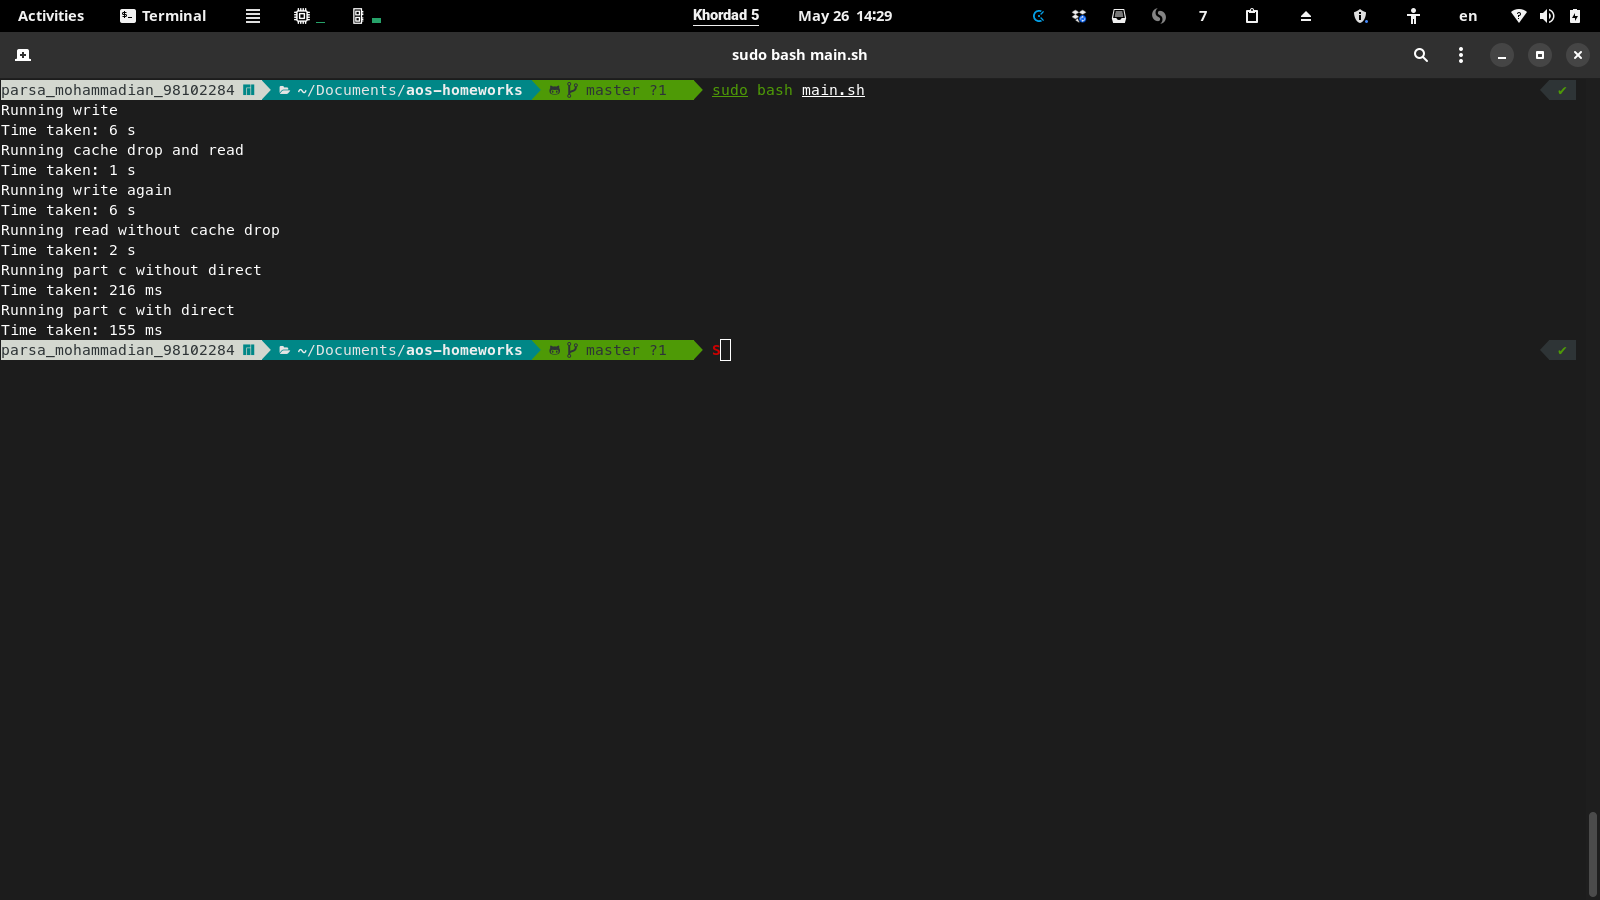
\includegraphics[width=\textwidth]{images/1.png}
\end{figure}

\subsection{}
در این قسمت برنامه اول ۶ ثانیه طول می‌کشد و برنامه دوم ۱ ثانیه. این به این معنا است 
که استفاده از فلگ 
\lr{direct}
عملیات خواندن را سریع‌تر می‌کند. دقت شود که در هر دو برنامه 
تنها زمان خواندن اندازه‌گیری شده است و در برنامه اول زمان عملیات نوشتن در نظر گرفته نشده است
تا بتوان مقایسه دقیق‌تری انجام داد.

\subsection{}
در اینجا کش را قبل از اجرای برنامه دوم پاک نمی‌کنیم. مشاهده می‌کنیم که 
برنامه اول همان ۶ ثانیه زمان برده است و برنامه دوم با وجود اینکه 
\lr{direct I/O}
است و نباید وابستگی به کش داشته باشد، ۲ ثانیه زمان می‌برد. 
به صورت کلی انگار با پاک نکردن کش، 
\lr{direct I/O}
زمان بیشتری طول می‌کشد. 

\subsection{}
در این قسمت مشاهده می‌کنیم که نوشتن با استفاده از کش 
۲۱۶ میلی ثانیه 
و نوشتن به صورت مستقیم ۱۵۵ میلی ثانیه طول می‌کشد.
نتیجه می‌گیریم که نوشتن به صورت 
\lr{direct}
سریع‌تر است ولی تاثیر آن کمتر از خواندن است. به عبارت دیگر تاثیر 
\lr{page cache}
در خواندن بیشتر مشاهده می‌شود.

\section{}
برنامه مربوط به نوشتن و خواندن فراداده به ترتیب در فایل‌های
\lr{2/write.c}
و
\lr{2/read.c}
قرار دارد. این دو برنامه نیاز به یک ورودی دارند که می‌تواند مقدار 
\lr{NOBUFFERCACHE}
یا
\lr{BUFFERCACHE}
را بپذیرد. این ورودی مشخص می‌کند 
آیا 
\lr{direct}
نوشته شود یا خیر. همچنین اسکریپت
\lr{2/main.sh}
کل کد‌ها را کامپایل و اجرا می‌کند. خروجی اجرای این اسکریپت را در قسمت زیر مشاهده می‌کنید.
توجه کنید که برای مقایسه بهتر، به جای ۱۰۰۰ فایل از ۱۰۰۰۰۰۰ 
استفاده شده است.

\begin{figure}[H]
    \centering
    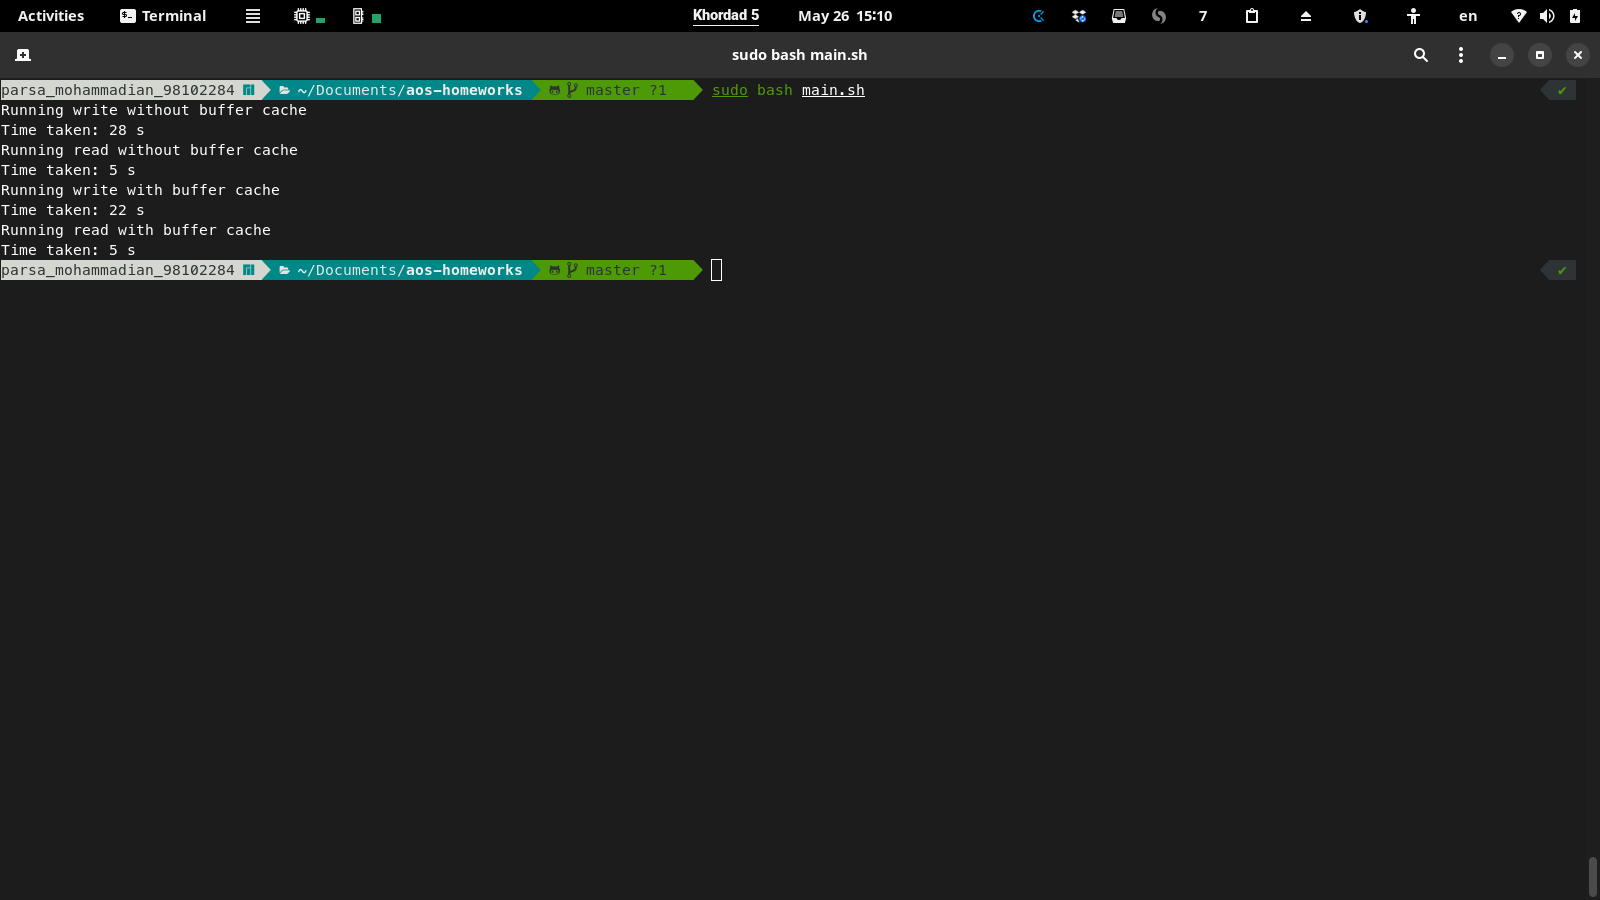
\includegraphics[width=\textwidth]{images/2.png}
\end{figure}

\subsection{}
همانطور که در شکل مشاهده می‌شود ۲۸ ثانیه طول می‌کشد.

\subsection{}
همانطور که در شکل مشاهده می‌شود 5 ثانیه طول می‌کشد.

\subsection{}
همانطور که در شکل مشاهده می‌شود 22 ثانیه طول می‌کشد.

\subsection{}
همانطور که در شکل مشاهده می‌شود 5 ثانیه طول می‌کشد.

\subsection{}
همانطور که از اعداد قابل درک است،‌ حافظه نهان میانگیر در خواندن فراداده 
تاثیر چندانی ندارد زیرا در هر دو حالت ۵ ثاینه زمان برده است. اما در نوشتن فراداده 
مشاهده می‌شود که استفاده از حافظه نهان میانگیر 
سبب کاهش ۶ ثانیه‌ای زمان یا به عبارت دیگر 
0/58
برابر شدن زمان می‌شود.

\section{}
در ابتدا ابزار 
\lr{Open CAS}
را نصب می‌کنیم.

\begin{figure}[H]
    \centering
    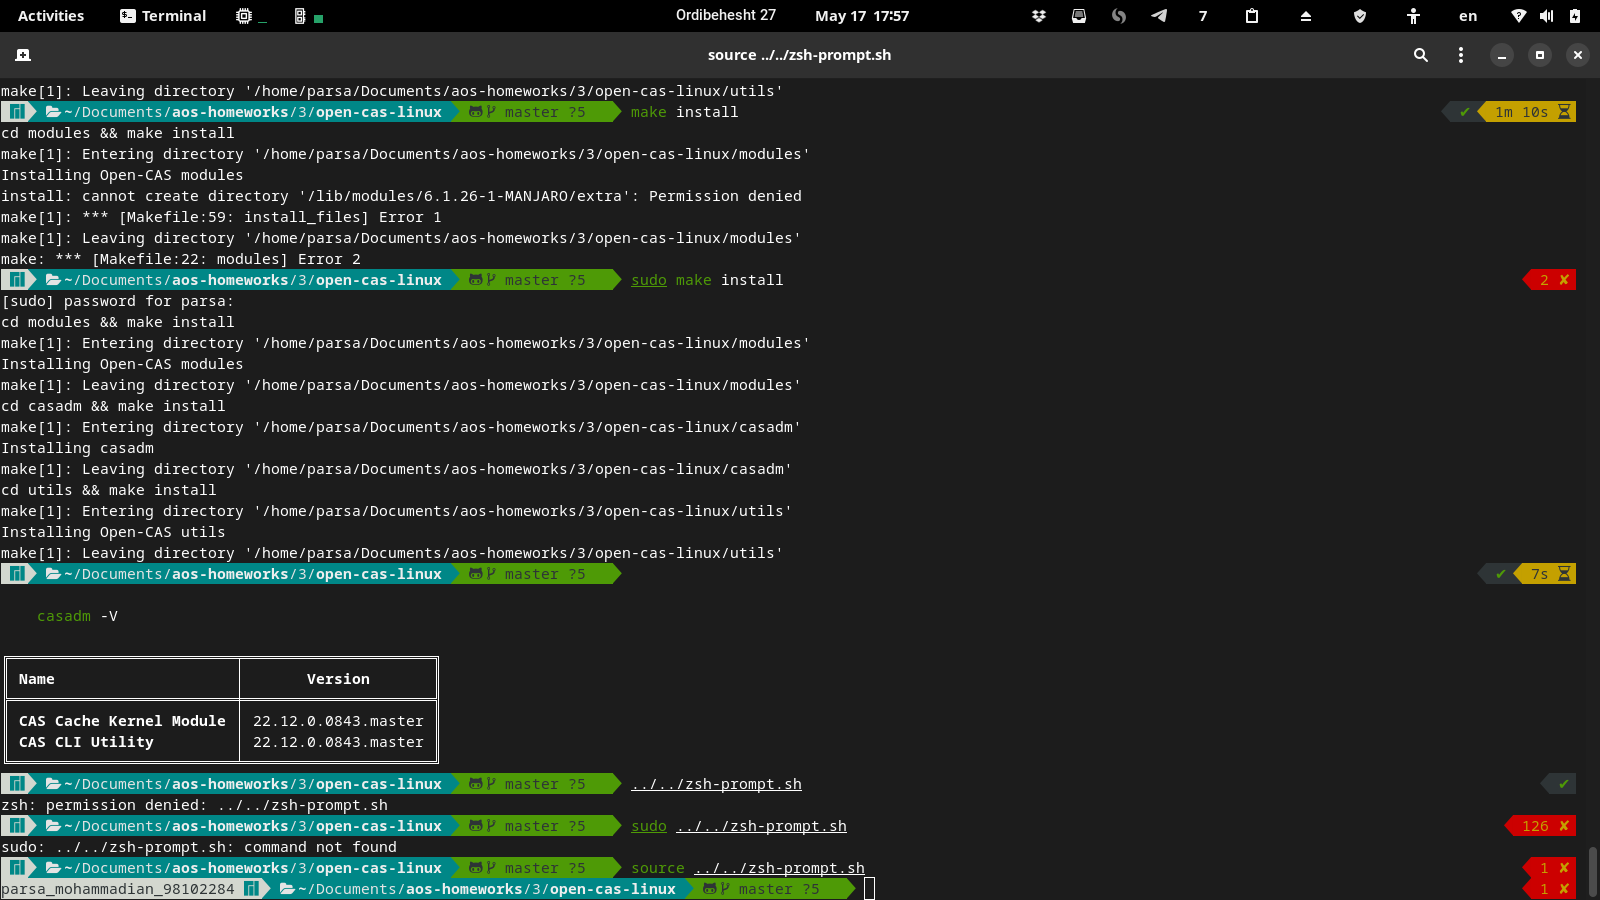
\includegraphics[width=\textwidth]{images/installing-open-cas.png}
\end{figure}

سپس ابزار 
\lr{fio}
را نصب می‌کنیم.

\begin{figure}[H]
    \centering
    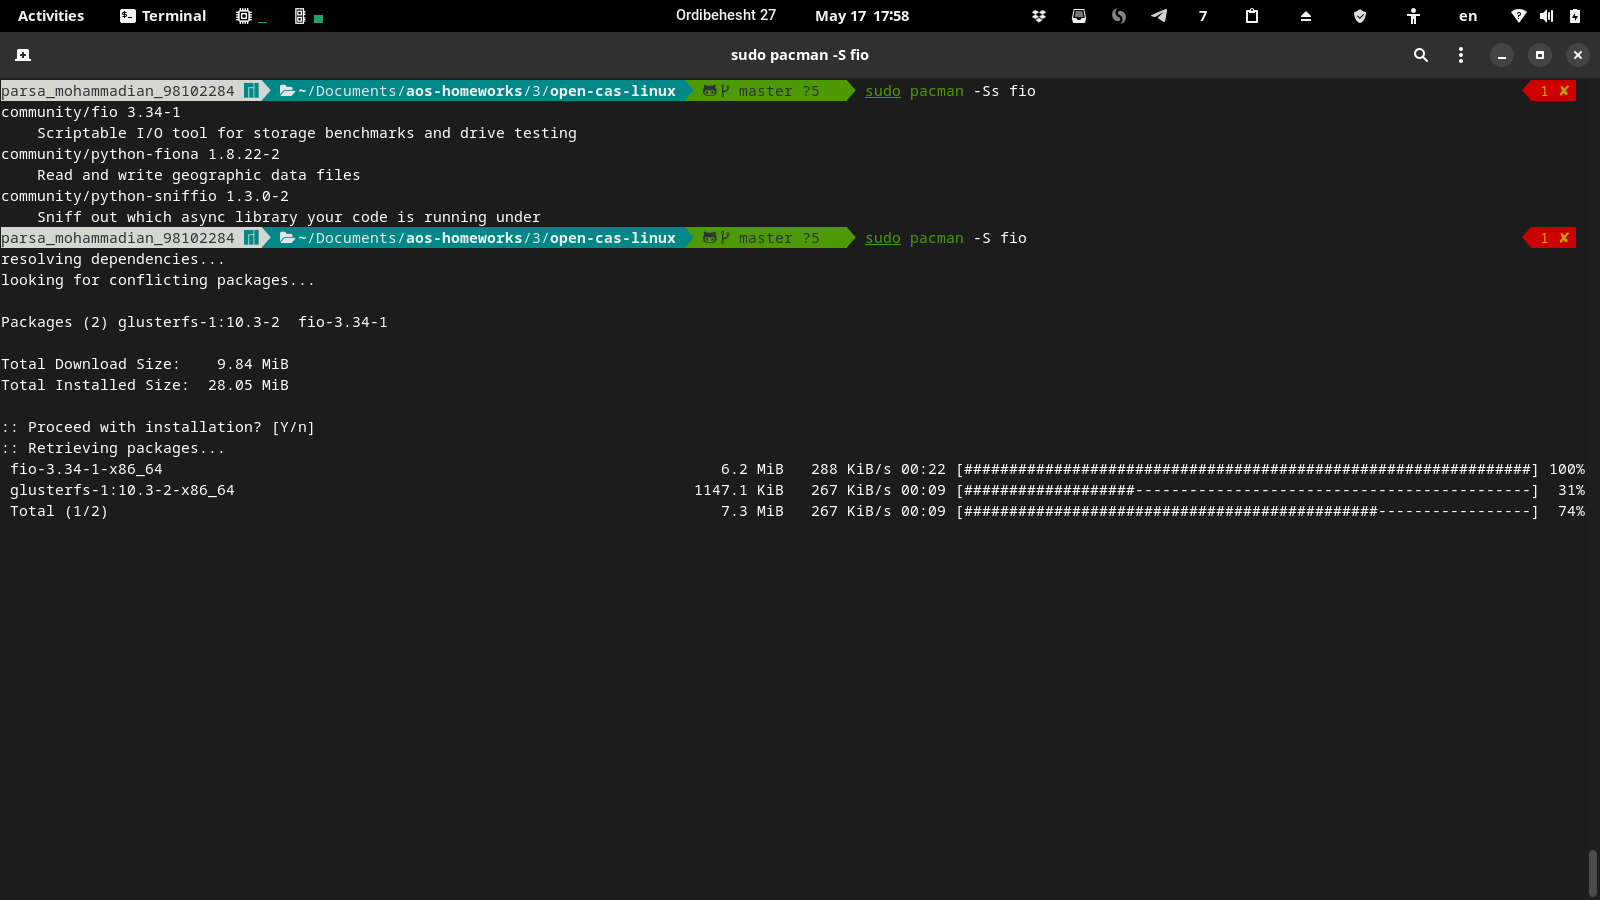
\includegraphics[width=\textwidth]{images/installing-fio.png}
\end{figure}

\subsection{}
همانطور که در شکل زیر مشاهده می‌شود، زمان اجرای دستور 
153
ثانیه است.

\begin{figure}[H]
    \centering
    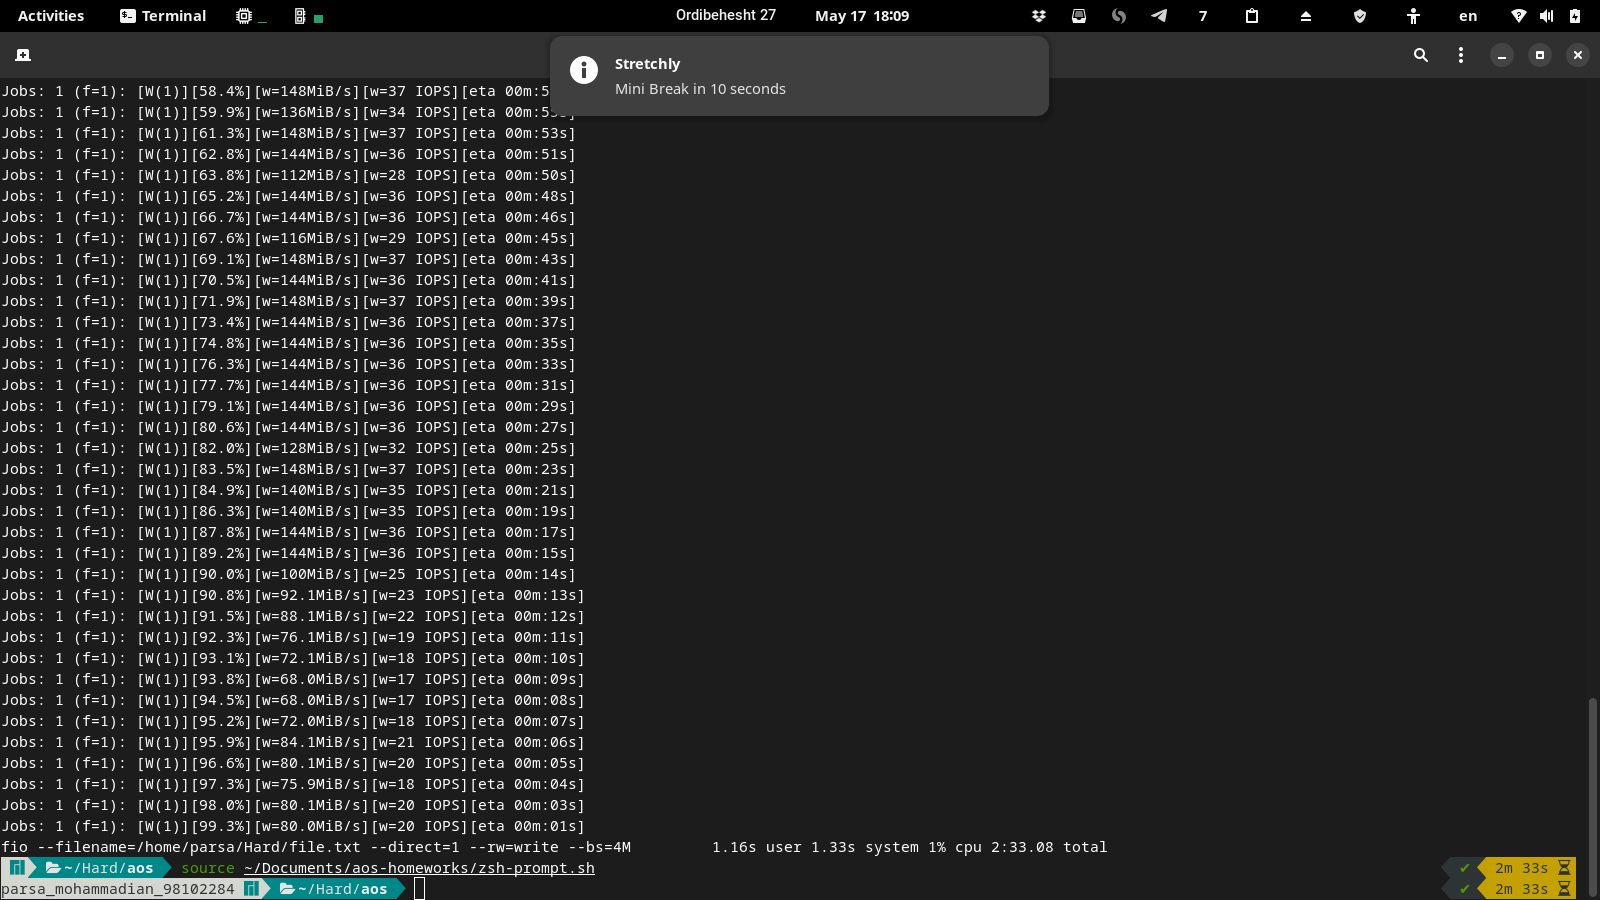
\includegraphics[width=\textwidth]{images/3-a.png}
\end{figure}

\subsection{}
همانطور که در شکل زیر مشاهده می‌شود، زمان اجرای دستور
148
ثانیه است.

\begin{figure}[H]
    \centering
    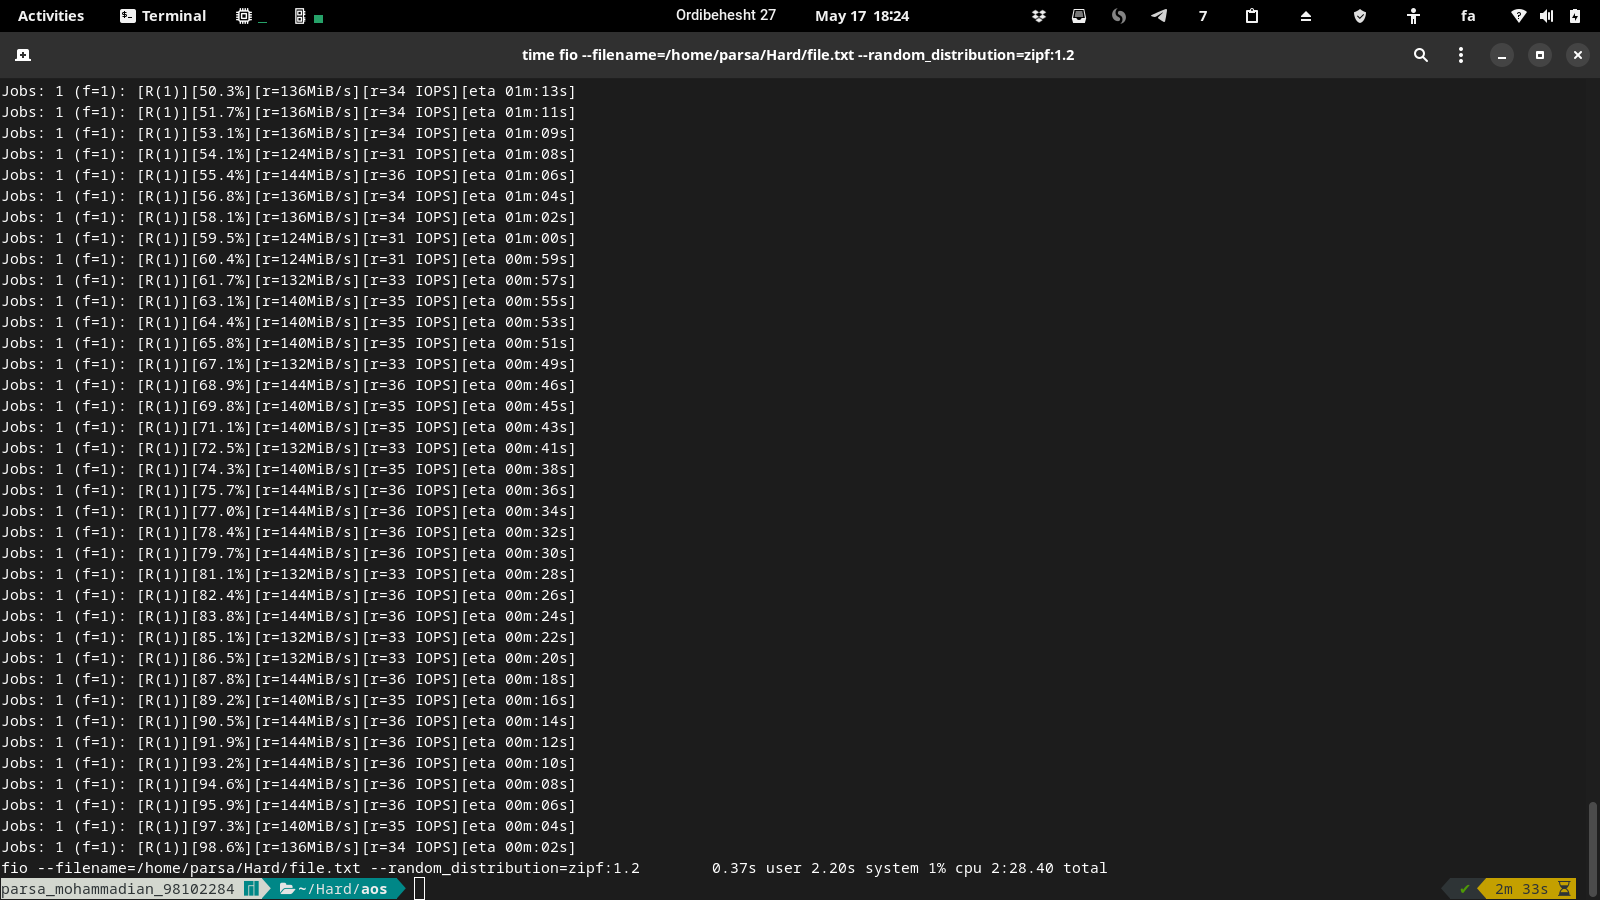
\includegraphics[width=\textwidth]{images/3-b.png}
\end{figure}

\subsection{}

در شکل زیر دستگاه‌های ذخیره‌ سازی سیستم را مشاهده می‌کنیم.

\begin{figure}[H]
    \centering
    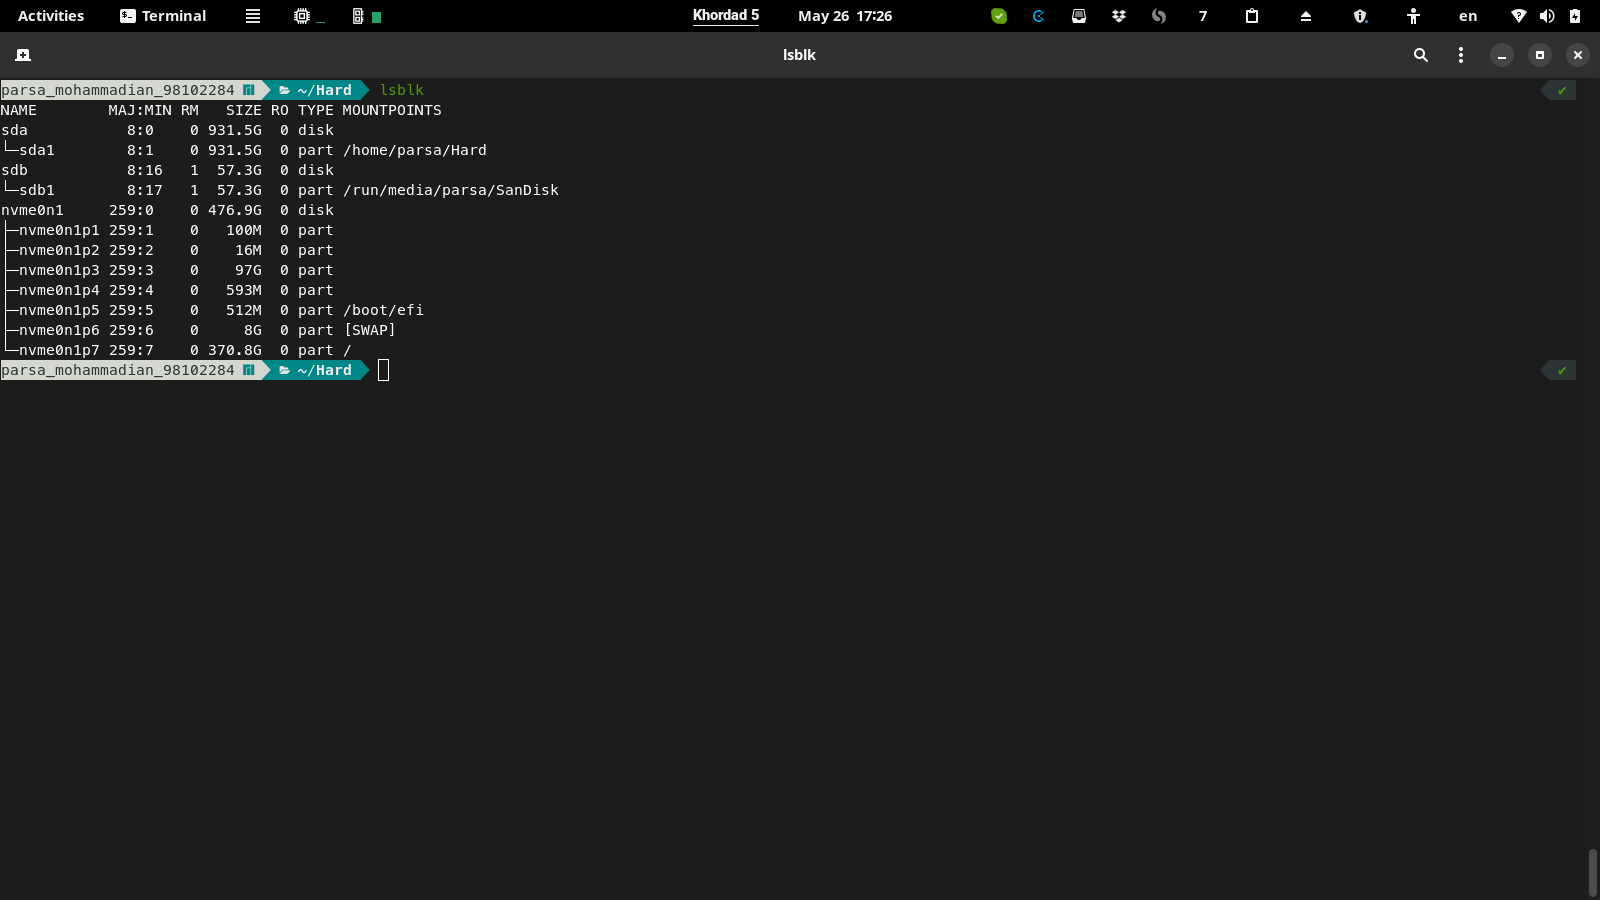
\includegraphics[width=\textwidth]{images/3-c-storage.png}
\end{figure}

در این قسمت به دلیل عدم در دسترس بودن 
\lr{SSD}،
از یک فلش به عنوان کش استفاده شده است.
همانطور که در تصویر زیر مشاهده می‌کنید سرعت فلش بالاتر از 
\lr{HDD}
است و در آزمایش تاثیر منفی ندارد.

\begin{figure}[H]
    \centering
    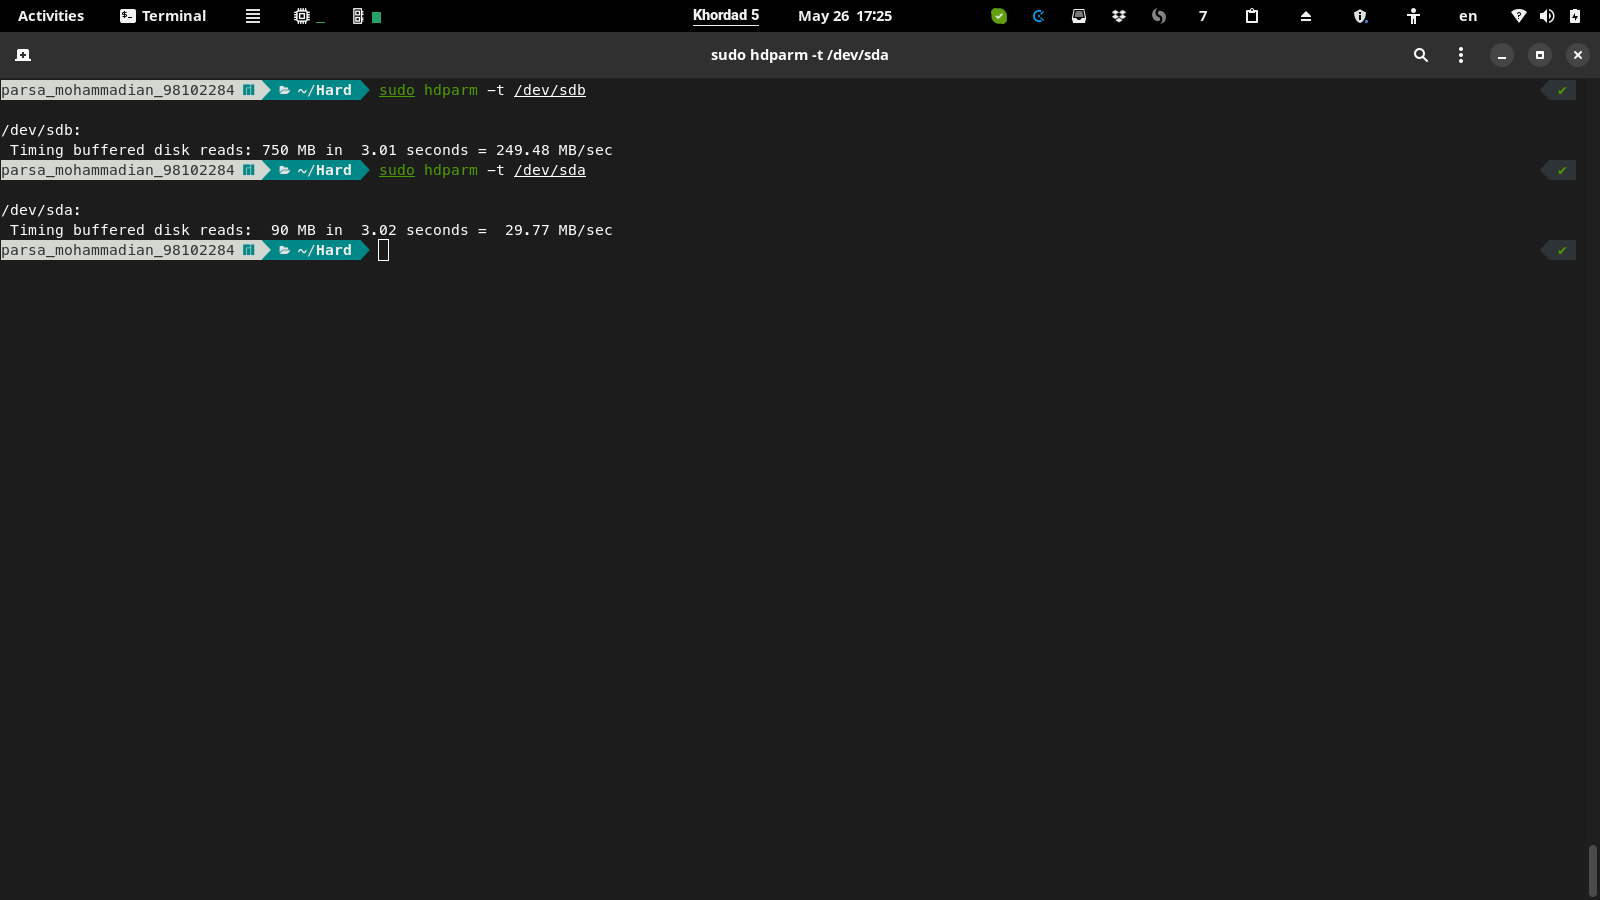
\includegraphics[width=\textwidth]{images/3-c-speed.png}
\end{figure}

حال با دستور زیر عملیات خواسته شده را انجام می‌دهیم.

\begin{latin}
\begin{lstlisting}
sudo casadm -S -d \
    /dev/disk/by-id/usb-USB_SanDisk_3.2\
    Gen1_01018cbcd5ec1843\
    a6ea309fc0300fc871ab1\
    edd6df237507244903575\
    23c3fa267000000000000\
    000000000f6a88cdaff82\
    500083558107652cfe4c-0:0 -i 1 -c wt --force
sudo casadm -A -d \
    /dev/disk/by-id/ata-TOSHIBA\
    _MQ04ABF100_28Q6PBRDT -i 1
sudo casadm -L
\end{lstlisting}
\end{latin}

اجرای دستورات بالا و خروجی دستور خواسته شده را در شکل زیر مشاهده می‌کنیم.

\begin{figure}[H]
    \centering
    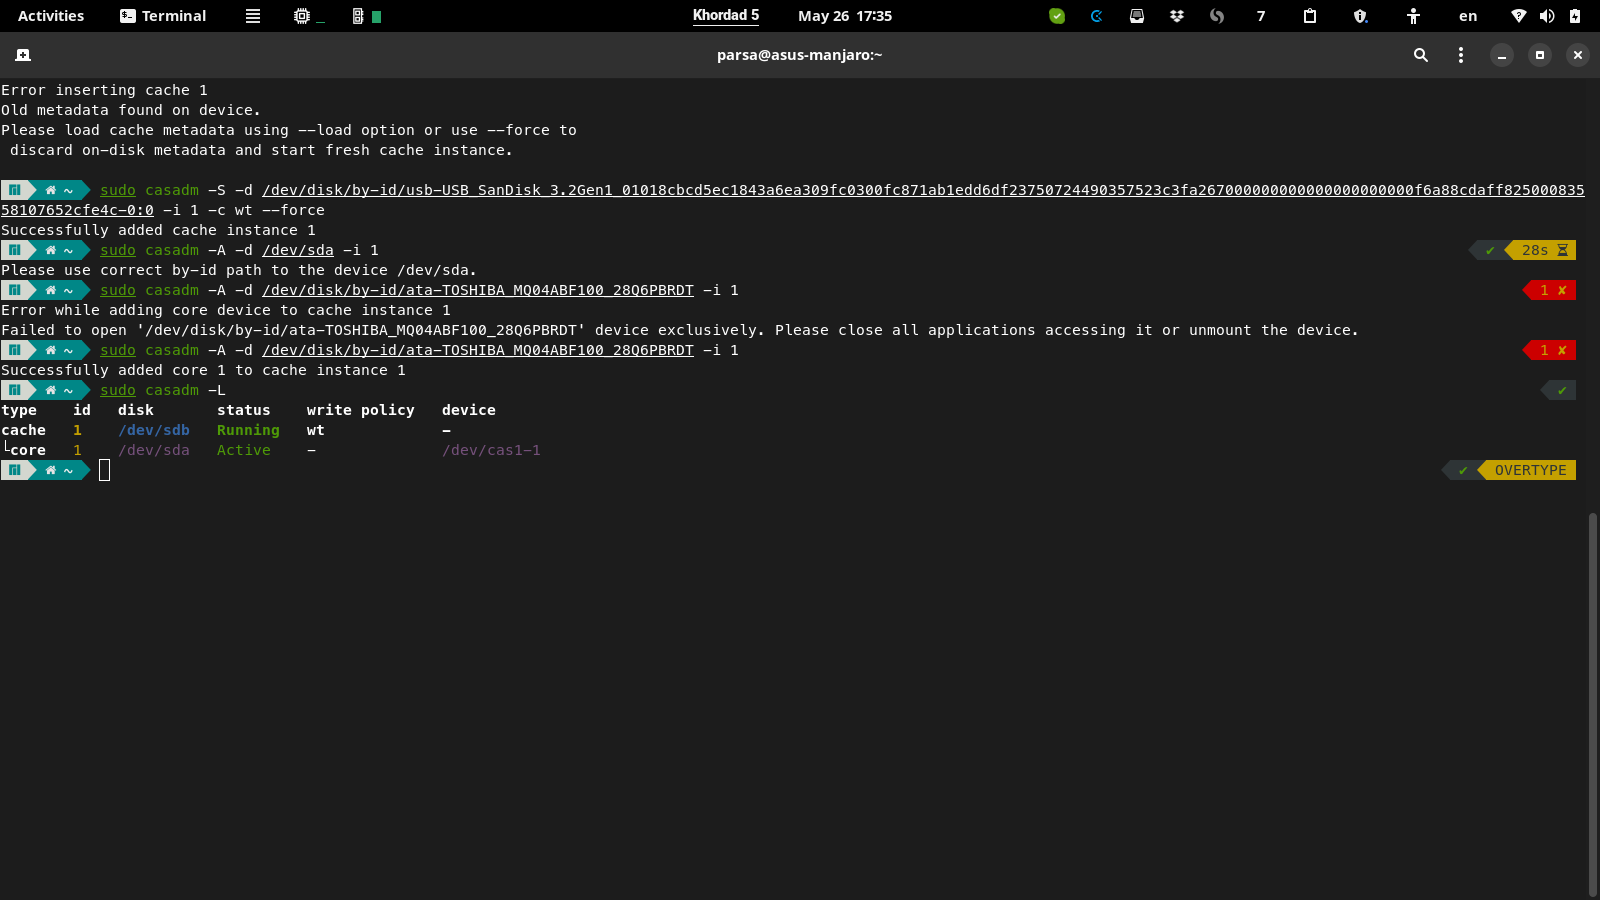
\includegraphics[width=\textwidth]{images/3-c-result.png}
\end{figure}

\subsection{}
\begin{itemize}
    \item سیاست \lr{Write-Through}
    در این سیاست، داده موقع نوشته شدن به صورت همزمان بر 
    \lr{cache}
    و
    \lr{backend storage}
    نوشته می‌شود. به همین دلیل خواندن در این حالت سریع‌تر است ولی نوشتن 
    عملا کندتر است زیرا در دو جا نوشته می‌شود.
    \begin{figure}[H]
        \centering
        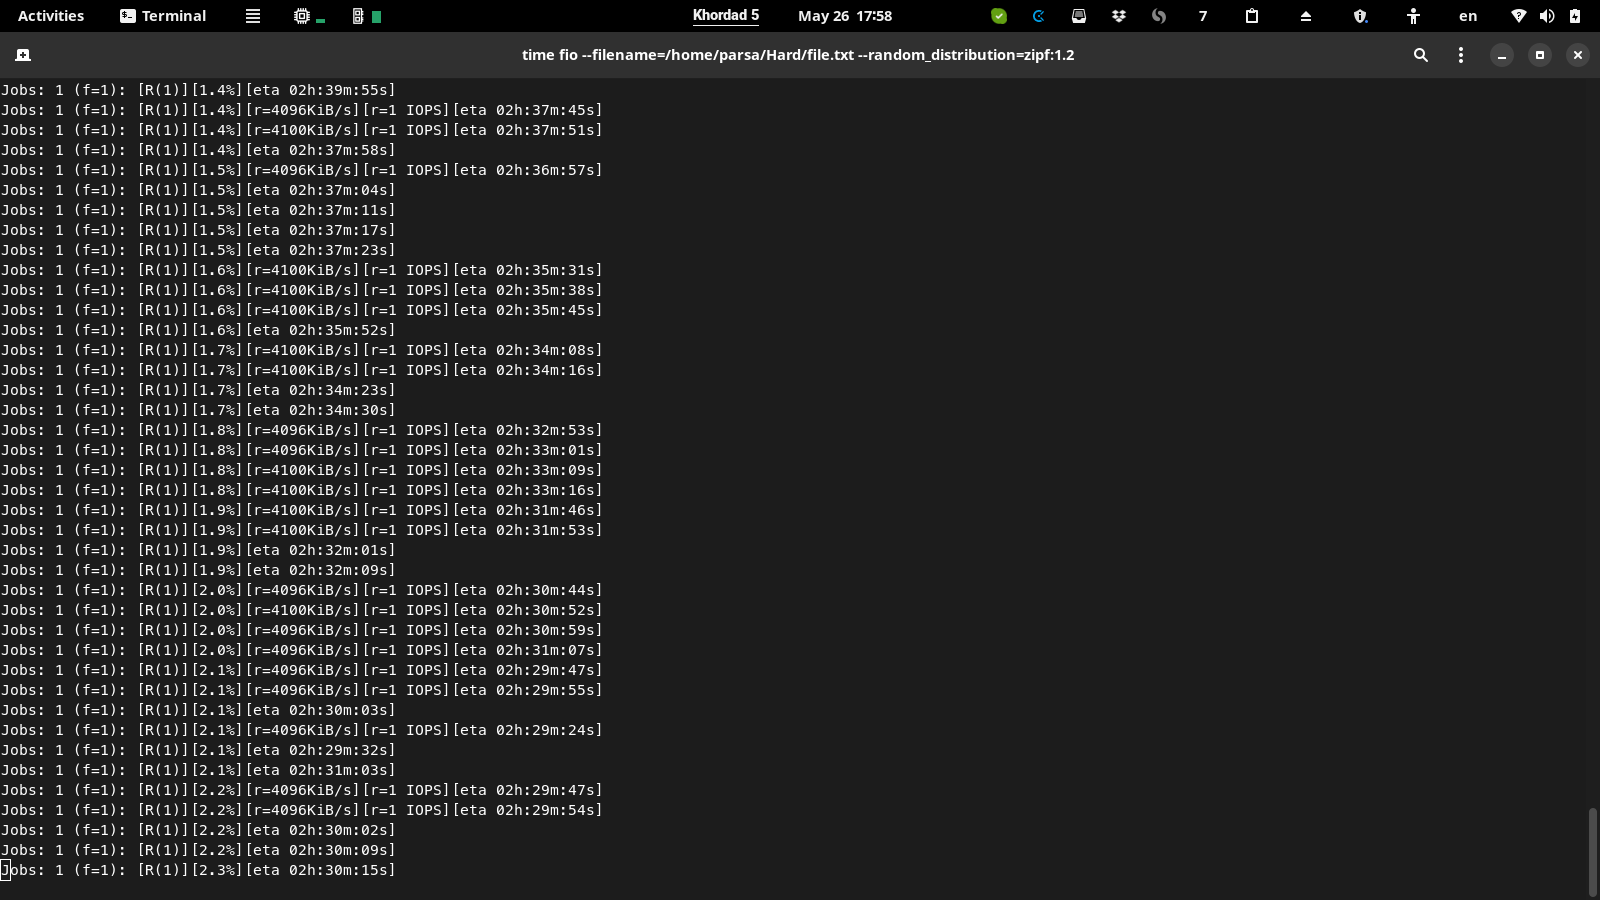
\includegraphics[width=\textwidth]{images/3-d-wt.png}
    \end{figure}
    \item سیاست \lr{Write-Back}
    در این سیاست، داده بر روی 
    \lr{cache}
    نوشته می‌شود و به اپلیکیشن گفته می‌شود که داده به صورت کامل نوشته شده.
    در حالی که داده بعدها به صورت دوره‌ای بر روی 
    \lr{backend storage}
    نوشته می‌شود. طبیعتا این روش سرعت خواندن و نوشتن را افزایش می‌دهد.
    \begin{figure}[H]
        \centering
        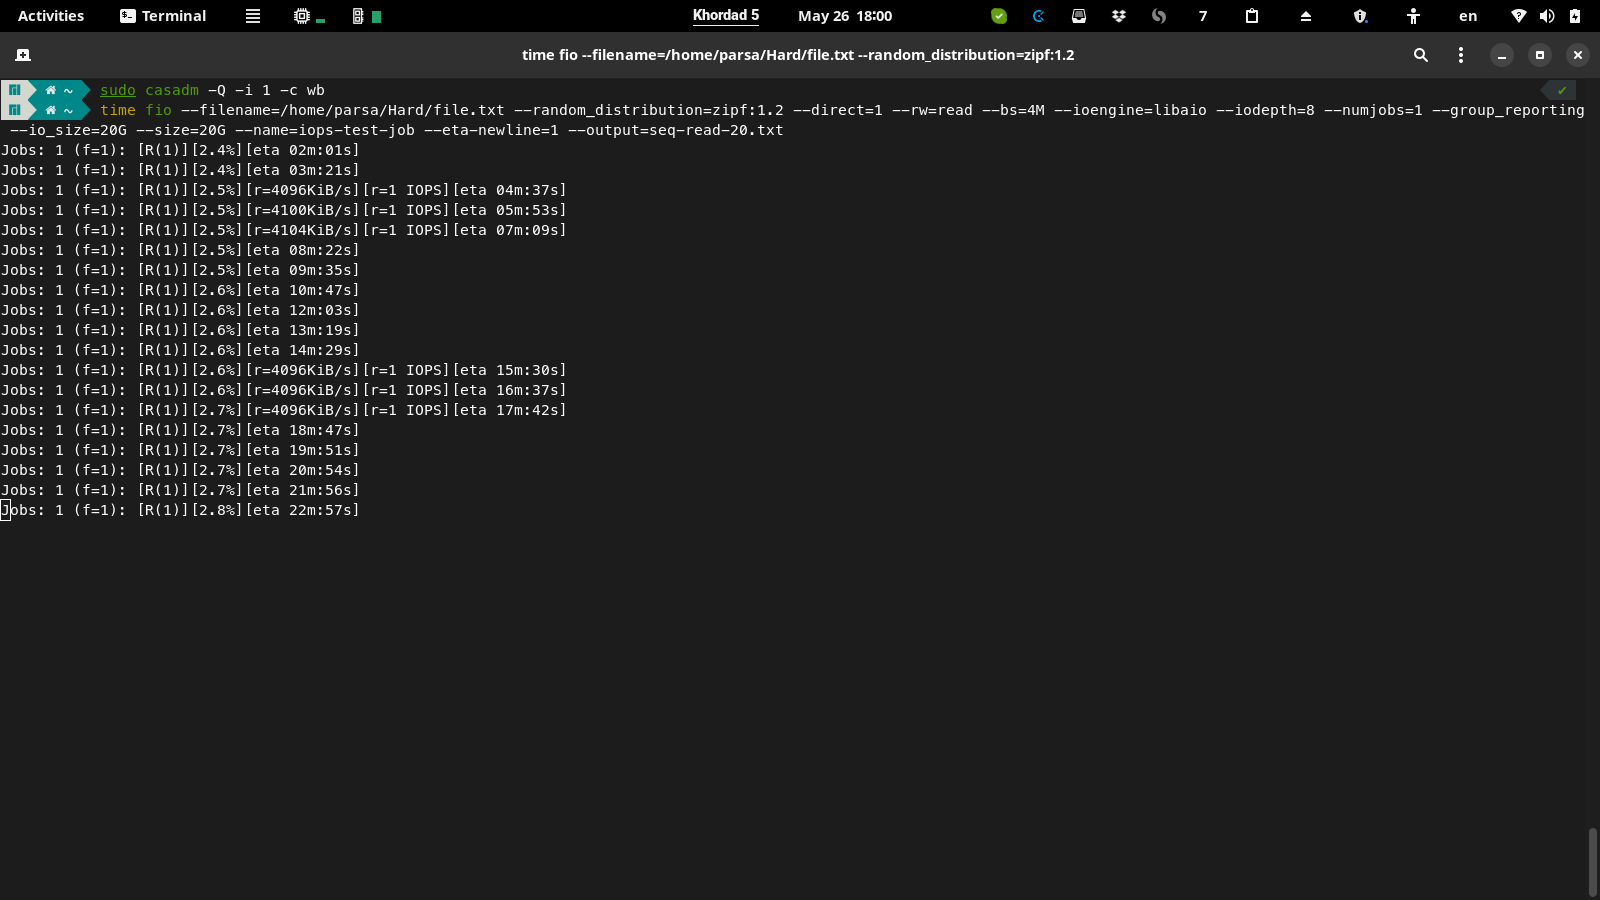
\includegraphics[width=\textwidth]{images/3-d-wb.png}
    \end{figure}
    \item سیاست \lr{Write-Around}
    این سیاست مانند 
    \lr{write through}
    عمل می‌کند با این تفاوت که تنها داده موجود در کش را موقع نوشتن آپدیت می‌کند.
    \begin{figure}[H]
        \centering
        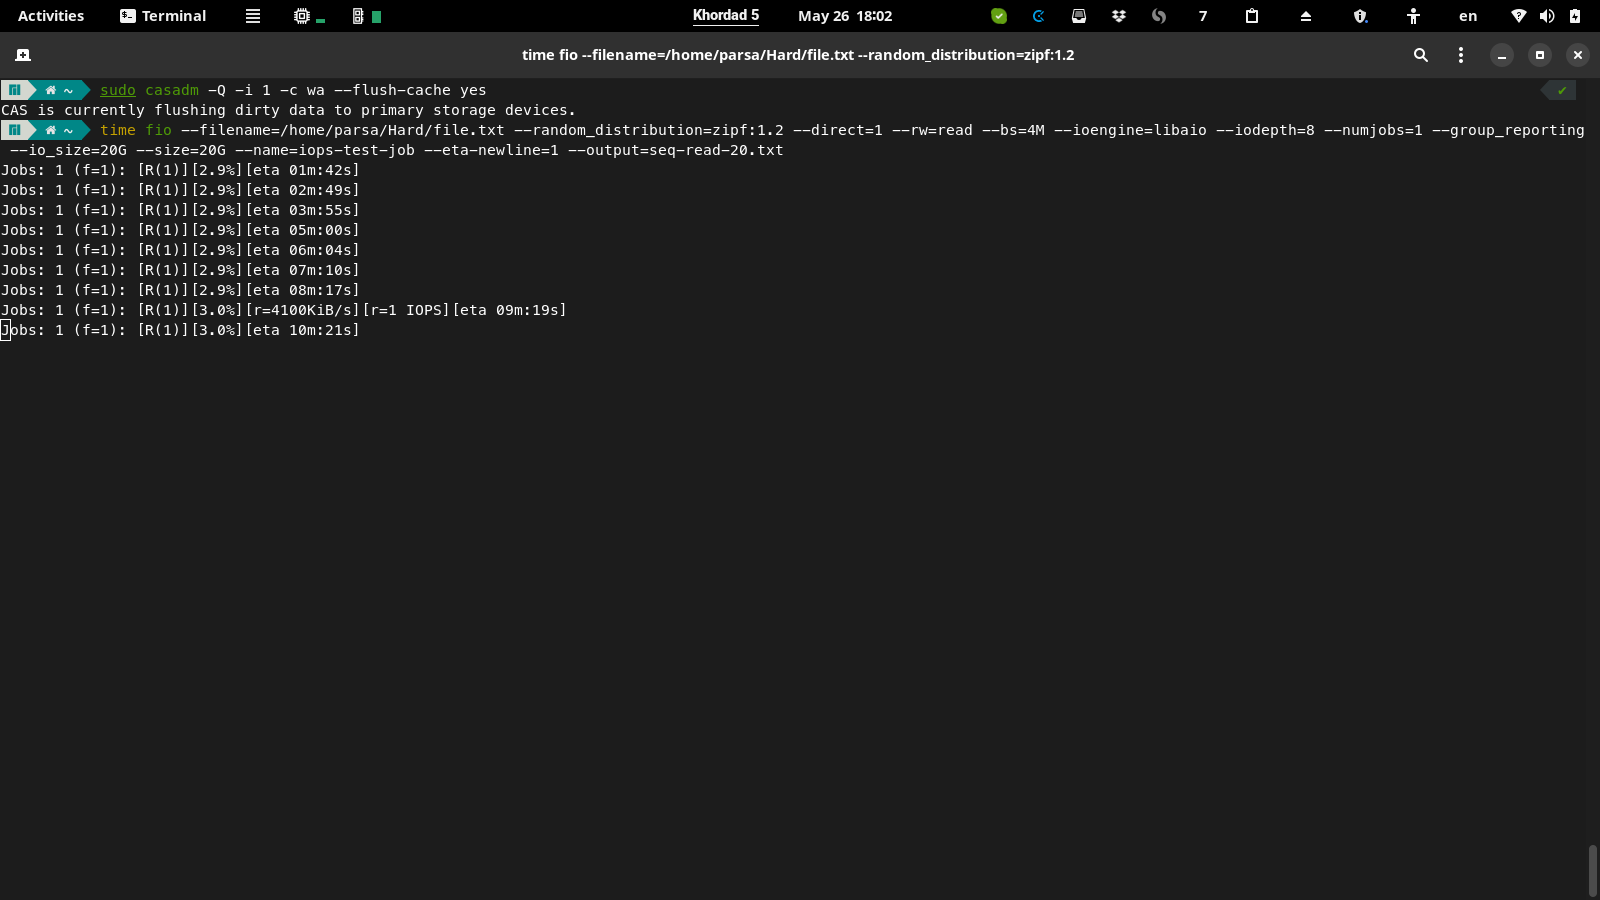
\includegraphics[width=\textwidth]{images/3-d-wa.png}
    \end{figure}
\end{itemize}

متاسفانه استفاده از فلش درایو به عنوان کش عملکرد خوبی ندارد. برای همین عملکرد 
تمامی سیاست‌ها برای کش ناکارآمد تر از قسمت ب شدند. ولی با این حال می‌توان 
سیاست‌های مختلف را با هم مقایسه کرد. 

همانطور که مشاهده می‌شود دو سیاست 
\lr{write back}
و 
\lr{write around}
تفاوت چندانی ندارند ولی سیاست 
\lr{write through}
نسبت به دو سیاست دیگر بسیار کند تر عمل می‌کند.

\subsection{}

\end{document}